\chapter[Normes]{Normes sur $\R^n$ et limites}
% Source: chapitre 1 du Nigio: Fonction de plusieurs variables
% ref/normes/evn.pdf
%
% To do: ajouter les compacts ? caractérisation séquentielle des fermés ?

\sld{\vfill\pagebreak[5]}%%%%%%%%%%%%%%%

\section{Normes et distances}
Le but de se chapitre est de formaliser et de donner un sens précis à l'assertion ``$x$ est proche de $y$'' quand $x,y\in \R^n$. On sait déjà mesurer les distances dans $\R^n$. Si $A=\begin{psmallmatrix}
    x_1\\\vdots\\x_n
\end{psmallmatrix}$ et $B=\begin{psmallmatrix}
    y_1\\\vdots\\y_n
\end{psmallmatrix}$
sont deux points de $\R^n$. La distance est différente suivant que l'on mesure la trajectoire
\begin{itemize}
    \item ``à vol d'oiseau'': c'est la distance $\ell^2$ ou euclidienne.
    \item ``taxi cab'': distance $\ell^1$ ou ``city norm''.
\end{itemize}

\sld{\vfill\pagebreak[5]}%%%%%%%%%%%%%%%

\subsection{Normes}

%Une norme est une fonctionnelle qui sert à mesurer des distances dans les espace vectoriels.

\begin{definition}
    Soit un \rev{} $E$. Une \emph{norme} est une application $N: E \to \R^+ = [0,\infty[$ qui vérifie les propriétés suivantes~:
            \begin{enumerate}
                \item Séparation: $\forall u \in E, N(u) \geq 0 \text{ et } N(u) = 0 \Leftrightarrow u=0$,
                \item 	Homogénéité: $\forall u \in E, \forall \lambda \in \R, N(\lambda u) = \abs{\lambda} N(u)$,
                \item  Inégalité triangulaire: $\forall (u,v) \in E^2, N(u+v) \leq N(u) + N(v)$.
            \end{enumerate}
        \end{definition}

        Dans la suite, on notera le plus souvent $N(\cdot) = \norm{\cdot}$. L'espace $E$ muni d'une norme $\norm{\cdot}$ est appelé un espace normé et est noté $(E,\ncd)$.
%Une norme est une fonctionnelle qui sert à mesurer la ``proximité'' de deux éléments de $E$. Plus précisément, le nombre $N(x-y)$ sera interprété comme la ``longueur'' (en fait la distance) du vecteur $x-y$. 


        \sld{\vfill\pagebreak[5]}%%%%%%%%%%%%%%%
        \begin{exemple}
            Si $E = \R^n$ et si $u = (x_1,\cdots,x_n)\in E$, on définit les normes usuelles suivantes~:
            \begin{enumerate}
                \item La norme 1 est $\norm{u}_1 = \abs{x_1} + \cdots + \abs{x_n} $
                    \pl{\rep{4cm} }
                \item La norme 2 est $\norm{u}_2 = \sqrt{x_1^2 + \cdots + x_n^2}$ dispose de propriétés particulières (norme euclidienne).
                \item La norme infinie est $\norm{u}_\infty = \max\{\abs{x_1},\cdots, \abs{x_n} \} $
                    \pl{\rep{4cm} }
            \end{enumerate}
        \end{exemple}

        \begin{proposition}
            Soit $(E,\ncd)$ un espace normé. On a pour tout $u,v\in E$
            \[
                \big\lvert\norm{u}- \norm{v}\big\rvert \leq \norm{u -v}.
            \]
        \end{proposition}
%\begin{remark}
%	On peut interpréter cette dernière propriété de la manière suivante: une norme est donc une application 1-Lipschitzienne et donc continue. Nous donnerons un sens précis à tout cela dans la suite, mais on peut dors et déjà comprendre 

%	Cette dernière inégalité nous apprend que si $x$ et $y$ sont proches au sens de la norme $N$ alors leur norme est proche (c'est à rapprocher du concept de continuité).
%\end{remark}
        \begin{proof}\sld{
%On a pour tout $u,v\in E$: $\norm{u} = \norm{u-v+v} \leq \norm{u-v} + \norm{v} $. Ainsi $\norm{u} - \norm{v} \leq \norm{u-v}$.
%	De même  $\norm{v} = \norm{v-u + u} \leq \norm{v-u} + \norm{u} $ et donc $ -\norm{u-v} \leq \norm{v} - \norm{u}$. Mis bout %à bout on a bien 
%	\[
%		-\norm{u-v} \leq \norm{u} - \norm{v} \leq \norm{u-v}.\qedhere
%	\]
            }
            \pl{\rep{6cm} }
        \end{proof}

        \sld{\vfill\pagebreak[5]}%%%%%%%%%%%%%%%
        \subsection{Distances}

        \begin{definition}
        %Soit un espace normé $\left( E, \ncd \right)$ et $a$ et $b$ deux points de $E$. On appelle distance de $a$ à $b$ (déduite de la norme $\ncd$) la quantité $d(a,b) = \norm{b-a}$.
            Soit $E$ un ensemble, une \emph{distance} est une application $d:E\times E \to [0,+\infty[$ telle que 
                    \begin{enumerate}
                        \item Symétrie: $\forall u,v \in E$ on a $d(u,v) = d(v,u)$
                        \item Séparabilité: $d(u,v) = 0$ si et seulement si $u=v$
                        \item Inégalité triangulaire: $\forall u,v,w\in E$ on a $d(u,w) \leq  d(u,v) + d(v,w)$
                    \end{enumerate}
                \end{definition}
                Un espace $E$ muni d'une distance $d$ est appelé espace métrique. On note $(E,d)$. Un espace normé est un espace métrique:

                \begin{proposition}
                    Si $(E,\ncd)$ est un espace normé. L'application $d:E\times E \to [0,+\infty[$ définie par $d(u,v) = \norm{u-v}$ est une distance sur $E$.
                        \end{proposition}
                        \begin{proof}
%	Laissé en exercice.
                            \pl{\rep{5cm}}
                        \end{proof}

                        \begin{remark}
                            Toutes les distances ne sont pas issues de normes: dans $E=\R$ on définit $d:\R\times \R \to \R$ par $d(x,y) = \operatorname{atan}(\abs{x-y})$. % atan est croissante et concave.
                            \pl{\rep{5cm}}
                        \end{remark}


                        \sld{\vfill\pagebreak[5]}%%%%%%%%%%%%%%%
                        \subsection{Boules ouvertes et fermées}

                        La notion de norme généralise la notion de valeur absolue dans $\R$ aux espaces vectoriels. La définition suivante généralise la notion d'intervalle ouvert et fermé dans $\R$ aux espaces vectoriels:  

                        \begin{definition}
                            Soit $(E,\ncd)$ un \rev{} normé, $a\in E$  et un nombre réel $r>0 $ fixé. L'ensemble 
                            \[
                            B_r(a) = \{ u \in E, \norm{u-a}<r \}\]  est appelé \emph{boule ouverte} de centre $a$ et de rayon $r$. L'ensemble \[\overline{B_r}(a) = \{ u \in E, \norm{u-a}\leq r \}\] est appelé \emph{boule fermée} de centre $a$ et de rayon $r$. 
                        \end{definition}

                        \sld{\vfill\pagebreak[5]}%%%%%%%%%%%%%%%
                        \begin{exemple}
                            Voici les boules unités fermées dans $E=\R^2$ pour:
                            \begin{center}
                                \begin{tabular}{ccc}
                                    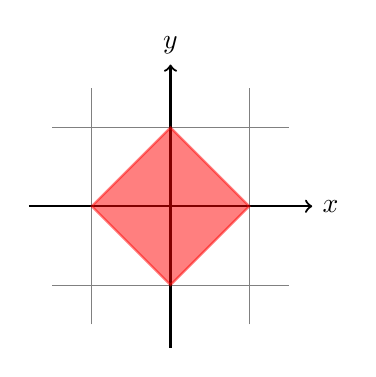
\begin{tikzpicture}
                                        \def\xone{-1.5};\def\xtwo{1.5};\def\yone{-1.5};\def\ytwo{1.5}

% grid
                                        \draw[step=1cm,help lines] (\xone,\yone) grid (\xtwo,\ytwo);
                                        \draw[thick,->] (\xone-.3, 0) -- (\xtwo+.3, 0) node[right] {$x$};
                                        \draw[thick,->] (0, \yone-.3) -- (0, \ytwo+.3) node[above] {$y$};
% ball
                                        \sld{	\draw[color=red,thick,fill=red, opacity=.5] (-1,0) -- (0,1) -- (1,0) -- (0,-1) -- cycle;}
                                    \end{tikzpicture}
                                    &
                                    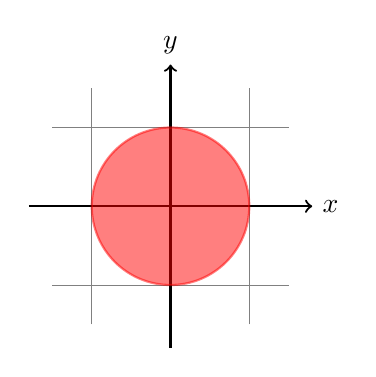
\begin{tikzpicture}
                                        \def\xone{-1.5};\def\xtwo{1.5};\def\yone{-1.5};\def\ytwo{1.5}
% grid
                                        \draw[step=1cm,help lines] (\xone,\yone) grid (\xtwo,\ytwo);
                                        \draw[thick,->] (\xone-.3, 0) -- (\xtwo+.3, 0) node[right] {$x$};
                                        \draw[thick,->] (0, \yone-.3) -- (0, \ytwo+.3) node[above] {$y$};
% ball
                                        \sld{
                                            \draw[color=red,thick,fill=red, opacity=.5] (0,0) circle (1cm);
                                        }
                                    \end{tikzpicture}&
                                    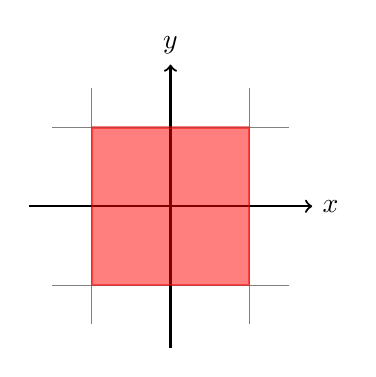
\begin{tikzpicture} 
                                        \def\xone{-1.5};\def\xtwo{1.5};\def\yone{-1.5};\def\ytwo{1.5};
% grid
                                        \draw[step=1cm,help lines] (\xone,\yone) grid (\xtwo,\ytwo);
                                        \draw[thick,->] (\xone-.3, 0) -- (\xtwo+.3, 0) node[right] {$x$};
                                        \draw[thick,->] (0, \yone-.3) -- (0, \ytwo+.3) node[above] {$y$};

% ball
                                        \sld{
                                            \draw[color=red,thick,fill=red, opacity=.5] (-1,-1) -- (-1,1) -- (1,1) -- (1,-1) -- cycle;
                                        }
                                    \end{tikzpicture}\\
                                    La norme $\ncd_1$
                                    & La norme $\ncd_2$
                                    & La norme $\ncd_\infty$
                                \end{tabular}
                            \end{center}
                        \end{exemple}

                        \sld{\vfill\pagebreak[5]}%%%%%%%%%%%%%%%
                        \begin{exemple}
                            Existe-t-il une norme dont la boule est l'un des ensembles suivants:
                            \begin{center}
                                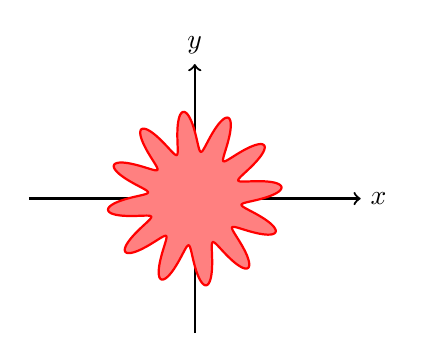
\begin{tikzpicture}
                                    \begin{axis}[height=3cm,xlabel = $x$,ylabel=$y$,height=5cm, axis equal,axis lines=middle, axis line style={->,thick}, xmin=-2,xmax=2,ymin=-2,ymax=2,xtick=\empty, ytick=\empty,every axis x label/.style={at={(current axis.right of origin)},anchor=west},every axis y label/.style={at={(current axis.above origin)},anchor=south},]
                                        \addplot[red,fill=red!50,samples=500, thick, domain = -pi:pi] ({cos(deg(x))*(1+ 0.3*sin(deg(12*x)))}, {sin(deg(x))*(1+ 0.3*sin(deg(12*x)))});
                                    \end{axis}
                                \end{tikzpicture}
                                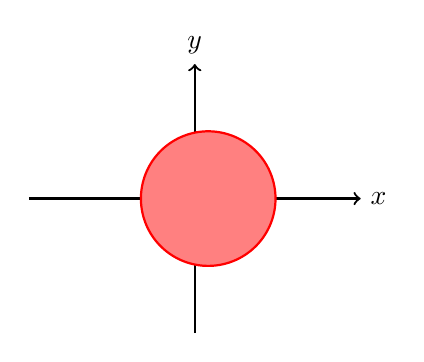
\begin{tikzpicture}
                                    \begin{axis}[height=3cm,xlabel = $x$,ylabel=$y$,height=5cm, axis equal,axis lines=middle, axis line style={->,thick}, xmin=-2,xmax=2,ymin=-2,ymax=2,xtick=\empty, ytick=\empty,every axis x label/.style={at={(current axis.right of origin)},anchor=west},every axis y label/.style={at={(current axis.above origin)},anchor=south},]
                                        \addplot[red,fill=red!50,samples=500, thick, domain = -pi:pi] ({cos(deg(x))+.2}, {sin(deg(x))});
                                    \end{axis}
                                \end{tikzpicture}
                                \begin{tikzpicture}
                                    \begin{axis}[height=3cm,xlabel = $x$,ylabel=$y$,height=5cm, axis equal,axis lines=middle, axis line style={->,thick}, xmin=-2,xmax=2,ymin=-2,ymax=2,xtick=\empty, ytick=\empty,every axis x label/.style={at={(current axis.right of origin)},anchor=west},every axis y label/.style={at={(current axis.above origin)},anchor=south},]
                                        \addplot[name path=F,red,domain={-3:3}] {1 +x};
                                        \addplot[name path=G,red,domain={-3:3}] {x-1};

                                        \addplot[red!50]fill between[of=F and G, soft clip={domain=-3:3}] ;

                                    \end{axis}
                                \end{tikzpicture}
                            \end{center}
                        \end{exemple}
                        \sld{\vfill\pagebreak[5]}%%%%%%%%%%%%%%%

                        \subsection{Normes équivalentes}

                        \begin{definition}[(Normes équivalentes)]
                            On dit que deux normes $\ncd$ et $\ncd': E\to\R$  sont équivalentes (et on note $\ncd \sim \ncd'$) s'il existe $\alpha>0$ et $\beta>0$ tels que, $\forall u \in E$
                            \[
                                \alpha \norm{u} \leq \norm{u}' \leq \beta \norm{u}
                            \]
                        \end{definition}

                        \begin{proposition}
                            La relation $\sim$ définit une relation d'équivalence sur les normes. 
                        \end{proposition}

                        \begin{proof}
                            \sld{
                %Soient $\ncd$, $\ncd'$ et $\ncd''$ trois normes sur $E$ alors la relation $\sim$ est~:
                %\begin{enumerate}
                        %\item Réflexive: on a $\ncd \sim \ncd$ en choisissant $\alpha = \beta =1$. 
                        %\item Symétrique: si $u\in E$ et $\alpha \norm{u} \leq \norm{u}' \leq \beta \norm{u}$ alors $\frac{1}{\beta} \norm{u}' \leq \norm{u} \leq \frac{1}{\alpha} \norm{u}'$.
                        %\item Transitive: si $u\in E$, $\alpha \norm{u} \leq \norm{u}' \leq \beta \norm{u} $  et $\alpha' \norm{u}' \leq \norm{u}'' \leq \beta' \norm{u}' $ alors $\alpha\alpha' \norm{u} \leq \norm{u}'' \leq \beta\beta' \norm{u} $.
                %\end{enumerate}
                            }
                            \pl{\rep{8cm}}
                        \end{proof}
                        \sld{\vfill\pagebreak[5]}%%%%%%%%%%%%%%%

                        \noindent On a l'interprétation géométrique suivante en termes de boules:
                        \begin{center}
                            \begin{tabular}{cc}
                                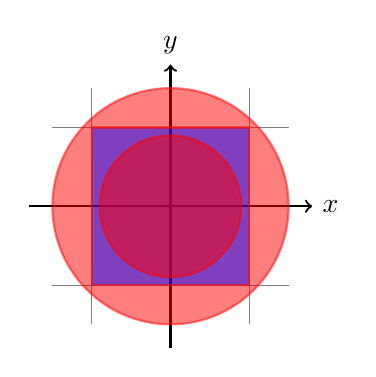
\begin{tikzpicture} 
                                    \def\xone{-1.5};\def\xtwo{1.5};\def\yone{-1.5};\def\ytwo{1.5};
% grid
                                    \draw[step=1cm,help lines] (\xone,\yone) grid (\xtwo,\ytwo);
                                    \draw[thick,->] (\xone-.3, 0) -- (\xtwo+.3, 0) node[right] {$x$};
                                    \draw[thick,->] (0, \yone-.3) -- (0, \ytwo+.3) node[above] {$y$};

% ball
                                    \draw[color=red,thick,fill=red,opacity=.5] (0,0) circle (1.5cm);
                                    \draw[color=red,thick,fill=blue,opacity=.5] (-1,-1) -- (-1,1) -- (1,1) -- (1,-1) -- cycle;
                                    \draw[color=red,thick,fill=red,opacity=.5] (0,0) circle (.9cm);

                                \end{tikzpicture} & 
                                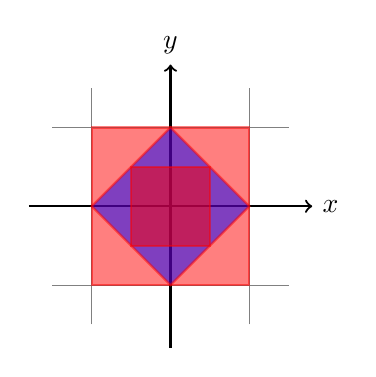
\begin{tikzpicture} 
                                    \def\xone{-1.5};\def\xtwo{1.5};\def\yone{-1.5};\def\ytwo{1.5};
% grid
                                    \draw[step=1cm,help lines] (\xone,\yone) grid (\xtwo,\ytwo);
                                    \draw[thick,->] (\xone-.3, 0) -- (\xtwo+.3, 0) node[right] {$x$};
                                    \draw[thick,->] (0, \yone-.3) -- (0, \ytwo+.3) node[above] {$y$};

% ball
                                    \draw[color=red,thick,fill=red,opacity=.5] (-1,-1) -- (-1,1) -- (1,1) -- (1,-1) -- cycle;
                                    \draw[color=red,thick,fill=blue,opacity=.5] (-1,0) -- (0,1) -- (1,0) -- (0,-1) -- cycle;
                                    \draw[color=red,thick,fill=red,opacity=.5] (-.5,-.5) -- (-.5,.5) -- (.5,.5) -- (.5,-.5) -- cycle;
                                \end{tikzpicture}
                                \\
                                $\ncd_2 \sim \ncd_\infty$
                                & $\ncd_\infty \sim \ncd_1$
                            \end{tabular}
                        \end{center}

                        \begin{theorem}
        %\label{}
                            Dans un \rev{} de dimension finie, toute les normes sont équivalentes.
                        \end{theorem}

                        \begin{proof}
                            Admis dans ce cours.
                        \end{proof}

                        \begin{remark}
                            Ce n'est pas vrai en dimension infinie. %Prendre $E = \mathcal C^1([0,1])$ avec $N_1$ et $N_\infty$.%mettre exemple C^1[0,1] du fichier /ref/normes/evn.pdf  page 5
                        \end{remark}

%\begin{proposition}
        %Les normes $N_1(\cdot),N_2(\cdot)$ et $N_\infty(\cdot)$ sont équivalentes sur $\R^n$.
%\end{proposition}

%\begin{proof}
%Il suffit de montrer que $N_\infty(x) \leq N_2(x) \leq N_1(x) \leq n N_\infty(x) $:
%\begin{itemize}
        %\item Tout d'abord:
                %\begin{align*}
                        %N_\infty(x) &= \left\{ \abs{x_1},\cdots,\abs{x_n} \right\} \\ 
                        %&= \sqrt{x_j^2} \qquad \text{(où $j$ est tel que $\abs{x_j} = N_\infty(x))$)}\\
                        %&= \sqrt{ x_1^2 + \cdots + x_n^2 } = N_2(x).
                %\end{align*}
        %\item \ldots puis:
%\begin{align*}			(N_2(x))^2 &= x_1^2 + \cdots+ x_n^2 \\ 
        %& \leq \abs{x_1}^2 + \cdots + \abs{x_n}^2 + 2 \sum_{1\leq i<j\leq n}\abs{x_i}\abs{x_j} \\ 
                        %&= ( \abs{x_1} + \cdots + \abs{x_n})^2 = (N_1(x))^2.
                %\end{align*}
        %\item \ldots et enfin
                %\begin{align*}
                        %N_1(x) &= \abs{x_1}+\cdots+\abs{x_n} \\
                        %& \leq n \max_{i=1,\ldots,n} \left\{ \abs{x_1},\cdots,\abs{x_n} \right\} \\
                        %& = n N_\infty(x).
                %\end{align*}
%\end{itemize}

%\end{proof}

                        \section{Limites de suites}

                        \begin{definition}[(Limite d'une suite)]
                            Soit $u=(u_k)_{k\in\N}$ une suite de points dans $(E,\ncd)$ et $\ell\in E$. On dit que la suite $u$ {converge} vers $\ell$ (ou la suite $u$ admet $\ell$ pour {limite}, ou $u$ tend vers $\ell$) au sens de la norme $\ncd$ si les conditions équivalentes suivantes sont satisfaites:
                            \begin{enumerate}
                                \item la suite de réels  $ \norm{u_{k} - \ell}$  tend vers 0 (\ie  $\lim_{k\to \infty} \norm{u_{k} -\ell} = 0$)
                                \item $\forall \varepsilon>0, \exists N\in\N, k\geq N \Rightarrow \norm{u_k - \ell} < \varepsilon$
                            \end{enumerate}
                        \end{definition}

                        \sld{\vfill\pagebreak[5]}%%%%%%%%%%%%%%%
                        \noindent Deux normes équivalentes ont les mêmes suites convergentes:
                        \begin{proposition}
                            Soit $E$ un \rev{} et $\ncd,\ncd': E \to [0,+\infty[$ deux normes équivalentes sur $E$. Pour toutes suites $(u_{k})_{k\in\N}$ et $\ell\in E$ les propriétés suivantes sont équivalentes:
                                    \begin{enumerate}
                                        \item $\lim_{k\to +\infty} u_{k} = \ell$ pour $\ncd$,
                                        \item $\lim_{k\to +\infty} u_{k} = \ell$ pour $\ncd'$.
                                    \end{enumerate}
                                \end{proposition}

                                \begin{proof}
                                    \pl{\rep{9cm}	}
                                \end{proof}

                                \sld{\vfill\pagebreak[5]}%%%%%%%%%%%%%%%
                                \noindent Dans $\R^n$ une suite converge si toutes les suites de ses coordonnées convergent:

                                \begin{proposition}
                                    Soit $u = (u_k)_{k\in\N} = \begin{psmallmatrix}u_{k,1}\\ \vdots \\ u_{k,n}\end{psmallmatrix}_{k\in\N}$ une suite de $\R^n$ et $\ell = \begin{psmallmatrix} \ell_1\\\vdots\\\ell_n\end{psmallmatrix} \in \R^n$. Alors les conditions suivantes sont équivalentes:
                                    \begin{enumerate}
                                        \item $\lim_{k\to +\infty} u_k = \ell$ dans $\R^n$
                                        \item Pour tout $i=1,\cdots,n$ on a  $\lim_{k\to +\infty} u_{k,i} = \ell_i$ dans $\R$
                                    \end{enumerate}
                                \end{proposition}

                                \begin{proof}
                                    \pl{\rep{8cm}	}

                                \end{proof}

                                \begin{remark}
                                    La limite est donc, si elle existe, unique.
                                \end{remark}

                                \sld{\vfill\pagebreak[5]}%%%%%%%%%%%%%%%
                                \section{Notions élémentaires de topologie}

                                \subsection{Ensembles ouverts et ensembles fermés}

                                \begin{definition}
                                    Soit $(E,\ncd)$ un \rev{} normé. On dit que 
                                    \begin{enumerate}
                                        \item une partie $\mathcal U$ de $E$ est un \emph{ouvert} pour la norme $\ncd$ si pour tout $a\in \mathcal U$, on peut trouver un réel $r>0$ tel que la boule $B_r(a) \subset \mathcal U$.  
                                        \item une partie $\mathcal F$ de $E$ est un \emph{fermé} pour la norme $\ncd$ si le complémentaire $E\setminus \mathcal F = \mathcal F^c = \left\{ u\in E| u \notin \mathcal F \right\}$ est une partie ouverte.
                                    \end{enumerate}
                                \end{definition}

                                \begin{exemple}
                                    \pl{\rep{5cm}	}
                                \end{exemple}

                                \sld{\vfill\pagebreak[5]}%%%%%%%%%%%%%%%
                                \begin{proposition}
                                Dans un \rev{} normé de dimension finie, une boule ouverte est un ouvert et une boule fermée est un fermé. \end{proposition}
                                \begin{proof}
                                    Soit $B_r(a)$ une boule ouverte de $\R^n$ et $x\in B_r(a)$. La boule $B_\rho(x)$ où $\rho = \frac{r - \norm{a -x}}{2}$ est incluse dans $B_r(a)$.
%\begin{center}
                                    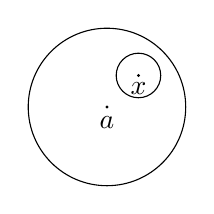
\begin{tikzpicture}
                                        \draw (0,0) node[below]{$a$} circle (0.01);
                                        \draw (0,0) circle (1cm);
                                        \draw (.4,.4) node[below=-1pt]{$x$} circle (0.01);
                                        \draw (.4,.4) circle (.2828);
                                    \end{tikzpicture}
%\end{center}
                                \end{proof}

                                \noindent Si deux normes sont équivalentes, alors les parties ouvertes (et fermées) sont les mêmes:
                                \begin{proposition}
                                    Soit $\mathcal U$ une partie d'un \rev{} $E$ et $\ncd$ et $\ncd'$ deux normes équivalentes sur $E$. La partie  $\mathcal U$ est un ouvert pour $\ncd$ si et seulement si $\mathcal U$ est un ouvert pour $\ncd'$.
                                \end{proposition}

                                \begin{proof}
                                    \pl{\rep{8cm}	}

                                \end{proof}


                                \begin{proposition}[(Caractérisation séquentielle des fermés)]
                                    Soit $\mathcal F$ une partie non vide d'un \rev{} normé $(E,\ncd)$. Les conditions suivantes sont équivalentes:
                                    \begin{enumerate}
                                        \item La partie $\mathcal F$ est fermée.
                                        \item Pour toute suite convergente de points de $\mathcal F$ alors la limite est dans $\mathcal F$.
                                    \end{enumerate}
                                \end{proposition}

                                \begin{proof}
                                    \pl{\rep{10cm}	}

                                \end{proof}

                                \sld{\vfill\pagebreak[5]}%%%%%%%%%%%%%%%
                                \subsection{Position d'un point}

                                \begin{definition}
                                    Soit $A$ une partie de $(E,\ncd)$ et $a\in E$. On dit que $a$ est un point
                                    \begin{enumerate}
                                        \item	\emph{Intérieur} à $A$ si on peut trouver un ouvert $\mathcal U \subset E$ tel que $a\in \mathcal U$ et $\mathcal U \subset A$. L'ensemble des points intérieurs à $A$ est noté $\mathring{A}$.
                                        \item	\emph{Adhérent} à $A$ si tout ouvert $\mathcal U \subset E$ qui contient $a$ satisfait $\mathcal U \cap A \neq \emptyset $. L'ensemble des points adhérents à $A$ est noté $\bar{A}$.
                                    \end{enumerate}
                                \end{definition}

                                \begin{center}
                                    \begin{tabular}{c}
                                        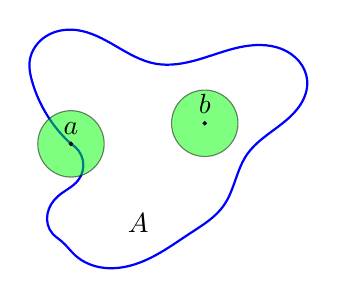
\begin{tikzpicture}[y=0.80pt, x=0.8pt,yscale=-1, scale=.3]
                                            \begin{scope}[]% layer1
  % path3029
                                                \path[,draw=blue,line join=miter,line cap=butt,line
                                                width=0.800pt] (98.5714,281.3729) .. controls (70.8127,256.1888) and
                                                (50.2769,223.1311) .. (40.0000,187.0872) .. controls (37.1535,177.1038) and
                                                (35.0669,166.6644) .. (36.4286,156.3729) .. controls (38.4655,140.9780) and
                                                (48.4007,127.1461) .. (61.6165,118.9916) .. controls (74.8322,110.8372) and
                                                (91.0080,108.1122) .. (106.4286,109.9443) .. controls (128.0218,112.5098) and
                                                (147.6221,123.3989) .. (166.4039,134.3576) .. controls (185.1857,145.3163) and
                                                (204.3205,156.7659) .. (225.7143,160.6586) .. controls (246.9864,164.5292) and
                                                (268.9327,160.5990) .. (289.7117,154.6226) .. controls (310.4907,148.6461) and
                                                (330.6998,140.6190) .. (351.8282,136.0281) .. controls (372.9566,131.4372) and
                                                (395.5974,130.4743) .. (415.6901,138.4597) .. controls (425.7365,142.4524) and
                                                (434.9733,148.6809) .. (441.9302,156.9558) .. controls (448.8871,165.2306) and
                                                (453.4851,175.5919) .. (454.2857,186.3729) .. controls (455.2115,198.8397) and
                                                (451.0656,211.3250) .. (444.3564,221.8733) .. controls (437.6472,232.4215) and
                                                (428.4885,241.2021) .. (418.7670,249.0615) .. controls (399.3239,264.7803) and
                                                (376.7905,277.7558) .. (362.8571,298.5157) .. controls (355.1132,310.0538) and
                                                (350.5022,323.3562) .. (345.9050,336.4696) .. controls (341.3077,349.5829) and
                                                (336.5511,362.8537) .. (328.5714,374.2300) .. controls (316.0601,392.0670) and
                                                (296.7907,403.7108) .. (278.5714,415.6586) .. controls (251.8717,433.1677) and
                                                (225.7667,452.6496) .. (195.4016,462.5190) .. controls (180.2191,467.4537) and
                                                (164.0573,469.8610) .. (148.1972,468.0391) .. controls (132.3371,466.2172) and
                                                (116.7890,459.9948) .. (105.0000,449.2300) .. controls (97.9078,442.7540) and
                                                (92.2774,434.7828) .. (85.0000,428.5157) .. controls (80.2575,424.4316) and
                                                (74.8328,421.0855) .. (70.7143,416.3729) .. controls (67.2344,412.3909) and
                                                (64.8038,407.5229) .. (63.5652,402.3817) .. controls (62.3267,397.2404) and
                                                (62.2694,391.8345) .. (63.2502,386.6379) .. controls (65.2118,376.2448) and
                                                (71.2992,366.8784) .. (79.2857,359.9443) .. controls (84.1039,355.7611) and
                                                (89.5750,352.4139) .. (94.8588,348.8368) .. controls (100.1426,345.2597) and
                                                (105.3244,341.3751) .. (109.2857,336.3729) .. controls (115.8694,328.0591) and
                                                (118.6048,316.8181) .. (116.5770,306.4089) .. controls (114.5492,295.9997) and
                                                (107.7944,286.6074) .. (98.5714,281.3729);

                                                \coordinate (a) at (98.5714,281.3729) ;
                                                \draw[fill=green,opacity=.5] (a)  circle (40pt);
                                                \draw[fill=blue,opacity=1] (a) node[above,opacity=1]{$a$}  circle (2pt);

                                                \coordinate (b) at (300,250.3729) ;
                                                \draw[fill=green,opacity=.5] (b)  circle (40pt);
                                                \draw[fill=blue,opacity=1] (b) node[above,opacity=1]{$b$}  circle (2pt);

                                                \node (A) at (200,400) {$A$};
                                            \end{scope}
                                        \end{tikzpicture}\\ 
                                        Le point $a$ est adhérent à $A$ et $b$ est intérieur à $A$.
                                    \end{tabular}
                                \end{center}

                                \begin{remark}
                                    La partie $\mathring{A}$ est ouverte et la partie $\bar A$ est fermée.
                                \end{remark}
                                \begin{exemple}
                                    \pl{\rep{9cm}	}
                                \end{exemple}

                                \sld{\vfill\pagebreak[5]}%%%%%%%%%%%%%%%
                                \subsection{Ensembles compacts}

                                \pl{Rappel sur les suites extraites\rep{5cm}}


                                \begin{definition}
                                    Une partie $\mathcal K$ d'un \rev{} $(E,\ncd)$ est dite \emph{compacte} si de toute suite de points de $\mathcal K$ on peut extraire une sous suite convergente dont la limite est dans $\mathcal K$.
                                \end{definition}
                                Autrement dit, toute suite de $\mathcal K$ admet une valeur d'adhérence dans $\mathcal K$.

                                \begin{theorem}
                                    [(Bolzano-Weierstrass)] Dans un \rev{} normé de dimension finie, les parties compactes sont les parties fermées bornées.
                                \end{theorem}

                                \begin{proof}
                                    Admise dans ce cours\ldots mais identique à la preuve dans le cas réel.
                                \end{proof}

                                \begin{exemple}
                                    \pl{\rep{3cm}	}
                                \end{exemple}

%\section{Limite d'une suite}

%\begin{definition}
        %Soit $\left( x_n \right)_{n\in\N}$ une suite de points de $\R^n$ et $\norm{\cdot}$ une norme. On dit que la suite $(x_n)$ a pour limite $\ell \in \R^n$ si 
        %$\forall \varepsilon >0, \exists n_0 \in \N$ ($n_0$ dépend de $\varepsilon$) tel que $n\geq n_0 \Rightarrow \norm{x_n - \ell } \leq \varepsilon$.
%\end{definition}

%Il existe des définitions équivalentes en termes de boules (ouvertes ou fermée) ou d'ouverts. Dans les espaces de dimension finie, la notion de limite et la limite elle même ne dépendent pas de la norme considérée. 
